\section{Идентификация объектов защиты в
  информационной системе фонда
  социального страхования}

\subsection{Цели и задачи фонда}

\point Цель деятельности фонда социального страхования~--- обеспечение
обязательного социального страхования граждан России.

\point Отделение фонда социального страхования осуществляет:

\begin{itemize}
\item выплату пособий по временной нетрудоспособности;
\item выплату пособий в связи с материнством и детством;
\item обеспечение социальными пособиями на погребение;
\item санаторно-курортное лечение. Оздоровление детей;
\item финансирование проведения углубленных медицинских осмотров
  работников занятых на работах с вредными и (или) опасными
  производственными факторами.
\end{itemize}

\point Функции фонда, которые могут быть автоматизированы с помощью
информационной системы: \label{functions}

\begin{enumerate}
\item организация банков данных по всем категориям страхователей;
\item ежеквартальный приём и выверка отчётных данных страхователей.
\end{enumerate}

\subsection{Идентификация информационных процессов}

В соответствии с функцией а) пункта~\ref{functions} можно
идентифицировать следующие информационные процессы.

\point Физическое или юридическое лицо, желающее зарегистрироваться в
качестве страхователя, отправляет с курьером (представителем
страхователя) на бумажном носителе заявление на регистрацию,
необходимые данные, а также документы, подтверждающие сферу
деятельности и уплату всех соответствующих налогов.

Получателем данной информации является специалист подразделения фонда,
ответственный за регистрацию страхователей.

\point На основе документов, предоставляемых физическим или
юридическим лицом, желающим зарегистрироваться в качестве
страхователя, специалист подразделения фонда, ответственного за
регистрацию страхователей (оператор), заносит необходимую информацию в
реестр (базу данных), добавляя к ней регистрационный номер и код
подчиненности. После чего с документов снимаются копии, которые вместе
с заявлением на регистрацию сдаются в архив. Подлинники документов
возвращаются страхователю.

\point Оператор получает доступ к информации, предоставленной
страхователем, но имеет право лишь на ввод её в базу данных. После
того, как данные о страхователе будут сохранены и отправлены по ЛВС на
сервер БД, единственным обладателем права доступа и модификации этих
данных становится администратор БД. Также в процессе осуществления
защитных мер к ним может получить доступ администратор ИБ.

\point Используемые программные приложения:

\begin{itemize}
\item программа для ввода данных о страхователе;
\item база данных HiTech;
\item ОС Windows.
\end{itemize}

\point Ввод информации осуществляется непосредственно на АРМ оператора,
последующая обработка и модификация~--- на АРМ администратора баз
данных.

Ввод данных с бумажных носителей в реестр, добавление регистрационного
номера и кода подчиненности осуществляется оператором вручную.

\point Обработанная информация в виде структурированной БД хранится на
сервере БД, а также на сервере резервного копирования. Доступ к
информации в БД осуществляется средствами запросов СУБД с АРМ
сотрудников фонда в соответствии с их должностными полномочиями.

В соответствии с функцией б) пункта~\ref{functions} можно
идентифицировать следующие информационные процессы.

\point Отчётные данные поступают от страхователя с курьером (представителем
страхователя) на бумажном носителе или через интернет (страхователь
после указания необходимых паролей может получить доступ через
интернет к своей отчётной информации в базе данных Фонда и прямо там
сформировать очередной ежеквартальных отчёт).

Отчёт исходит от бухгалтера страхователя к оператору ИС Фонда.

\point Если отчёт поступает с курьером на бумажном носителе,
специалист Фонда (оператор) на своём рабочем месте осуществляет ручной
ввод информации в базу данных (данные приводятся к формализованному
виду), которая хранится на сервере баз данных.

Если отчёт поступает через интернет, то он обрабатывается
автоматически. В данном случае к информации получают доступ сам
оператор, администратор баз данный.

\point Используемые программные приложения:

\begin{itemize}
\item программа для ввода данных отчёта;
\item база данных HiTech;
\item ОС Windows.
\end{itemize}

\point Отчётные данные страхователя заносятся в базу данных
специалистом фонда или автоматически.

\point После обработки, отчётные данные страхователя представлены в
формализованном виде и хранятся в базе данных, доступ к которой
(удаление, модификация) может осуществлять администратор баз данных с
использованием СУБД HiTech.

\subsection{Структура ИС фонда}

\point Информационная система фонда состоит из следующих элементов:

\begin{enumerate}
\item серверная ферма:
  \begin{enumerate}
  \item почтовый сервер;
  \item сервер обработки, на котором установлена СУБД;
  \item сервер резервного копирования.
  \end{enumerate}
\item Автоматизированные рабочие места:
  \begin{enumerate}
  \item операторов;
  \item администратора БД (резервного копирования);
  \item администратора почтового сервера;
  \item администратора ИБ.
  \end{enumerate}
\item Сетевое оборудование:
  \begin{enumerate}
  \item коммутатор;
  \item маршрутизатор.
  \end{enumerate}
\end{enumerate}

\point Графическое изображение конфигурации системы представлено на
рисунке:

\begin{figure}[h]
  \centering
  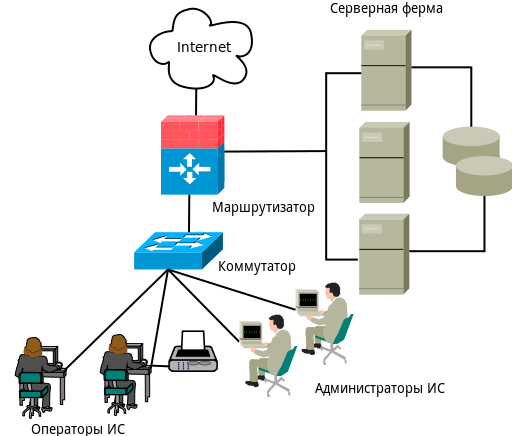
\includegraphics[width=\textwidth]{Structure}
  \caption{Конфигурация информационной системы фонда социального страхования}
  \label{fig:structure}  
\end{figure}

\subsection{Идентификация аппаратных ресурсов
  фонда как объектов защиты}

\point Следующим этапом курсовой работы является определение
ответственных за каждый аппаратный ресурс ИС и их полномочия по
отношению к этим ресурсам с точки зрения возможности изменения
конфигурации этих ресурсов. Для каждого аппаратного ресурса
определяются его пользователи и их полномочия тоже с точки зрения
возможности изменения конфигурации этих ресурсов, т.~е. происходит
идентификация аппаратных ресурсов как объектов защиты с указанием
возможных источников угроз для них.

\point Результат представлен в таблице~\ref{hardware}
Приложения~\ref{AppendixA}.

\subsection{Идентификация информационных ресурсов
  фонда как объектов защиты}

\point На следующем этапе курсовой работы необходимо идентифицировать
информационные ресурсы, подлежащие защите. 

\point В таблице~\ref{tab:inf_resource} представлена классификация
информационных русурсов по степени критичности относительно
доступности, целостности и конфиденциальности.

\begin{table}[h]
\caption{Классификация ИР фонда по степени критичности}
\label{tab:inf_resource}
\small
\begin{tabular}{|p{5cm}|p{3cm}|p{3cm}|p{3cm}|}
\hline
\multirow{3}{4cm}{Информационный ресурс} & \multicolumn{3}{c|}{Степень
  критичности информации}\\\cline{2-4}
& Доступность & Целостность & Конфиденциаль\-ность \\\hline
Документы, необходимые для регистрации страхователя & Важная & Важная
& Значимая\\\hline
Отчётные данные страхователя на бумажном носителе & Важная & Важная &
Значимая \\\hline
Отчётные данные страхователя в электронном виде & Важная & Важная &
Значимая \\\hline
Содержимое сервера БД & Критическая & Критическая & Очень важная
\\\hline
Резервная копия БД & Важная & Очень важная & Очень важная
\\\hline
\end{tabular}
\end{table}
\normalsize

\point В таблице~ Приложения~\ref{AppendixA} определяются
ответственные за информационные ресурсы фонда, их пользователи, а
также как ответственные и пользователи используют информационные
ресурсы.



%%% Local Variables: 
%%% mode: latex
%%% TeX-master: "../TermWork_OPOIB"
%%% End: 
